\documentclass{beamer}

\usepackage{amsmath}
\usepackage{amssymb}
\usepackage{centernot}
\usepackage{graphics}
\usepackage{hyperref}
\usepackage{listings}
\usepackage{setspace}
\usepackage{tikz}
\usepackage{xcolor}


\newcommand{\shrug}[1][]{%
\begin{tikzpicture}[baseline,x=0.8\ht\strutbox,y=0.8\ht\strutbox,line width=0.125ex,#1]
\def\arm{(-2.5,0.95) to (-2,0.95) (-1.9,1) to (-1.5,0) (-1.35,0) to (-0.8,0)};
\draw \arm;
\draw[xscale=-1] \arm;
\def\headpart{(0.6,0) arc[start angle=-40, end angle=40,x radius=0.6,y radius=0.8]};
\draw \headpart;
\draw[xscale=-1] \headpart;
\def\eye{(-0.075,0.15) .. controls (0.02,0) .. (0.075,-0.15)};
\draw[shift={(-0.3,0.8)}] \eye;
\draw[shift={(0,0.85)}] \eye;
% draw mouth
\draw (-0.1,0.2) to [out=15,in=-100] (0.4,0.95); 
\end{tikzpicture}}


\lstset{basicstyle=\ttfamily\footnotesize,language=Bash,showstringspaces=false}


\title{An Introduction to Singularity: \\
       \small Containers for Scientific and High-Performance Computing}
\author{Marty Kandes, Ph.D. \\ \ \\
   \small High-Performance Computing User Services Group \\
          San Diego Supercomputer Center \\
          University of California, San Diego}
\date{\small SDSC Summer Institute 2020 \\
             Friday, August 7th, 2020 \\
             8:30AM - 9:00PM PDT}

\begin{document}
\maketitle

\begin{frame}
   \frametitle{Today's Session}
   \begin{itemize}
      \setlength\itemsep{1.0em}
      \item What are containers? And why you should use them.
      \item What is Singularity and what does it have to do with containers?
      \item How to build and run Singularity containers.
      \item Q\&A?
   \end{itemize}
\end{frame}

\begin{frame}
   \frametitle{Containers}
   \vspace{-1.0em}
   \begin{figure}[htbp]
      \includegraphics[width=0.9\textwidth]{images/containerization-shipping-loading-binary-code-data-containers-orig.jpg}
   \end{figure} 
\end{frame}

\begin{frame}
   \frametitle{What is a Container?}
   \begin{columns}
      \begin{column}{0.6\textwidth}
         \begin{itemize}
            \setlength\itemsep{1.0em}
            \item At rest, a container or \textbf{container image} is 
               simply a file (or collection of files) saved on disk that 
               stores everything you need to run a target application or 
               applications: code, runtime, system tools, libraries and 
               settings, etc.
            \item \textit{In motion}, a container or \textbf{container 
               process} is simply a standard (Linux) process running on
               top of the underlying host's operating system and kernel, 
               but whose software environment is defined by the contents 
               of the container image.
         \end{itemize}
      \end{column}
      \hfill
      \begin{column}{0.5\textwidth}
         \begin{figure}[htbp]
            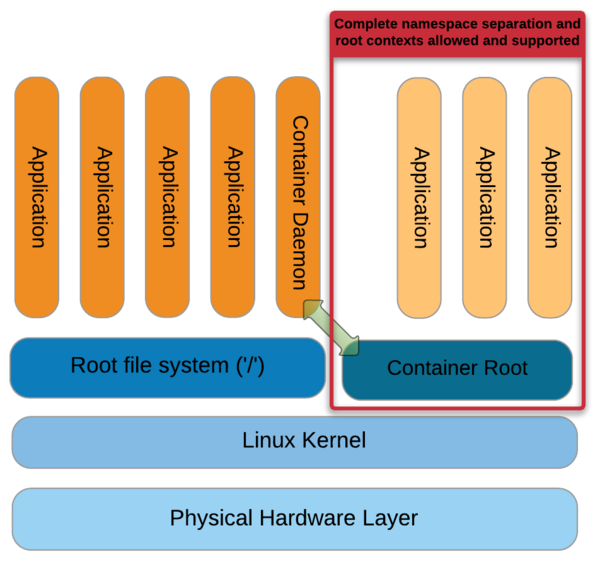
\includegraphics[width=1.0\textwidth]{images/singularity-generic-container-architecture.png}
         \end{figure}
      \end{column}
   \end{columns}
\end{frame}

\begin{frame}
   \frametitle{Container : Supercomputer :: Construct : Matrix}
   `` ... it's our loading program.''
   \begin{figure}[htbp]
      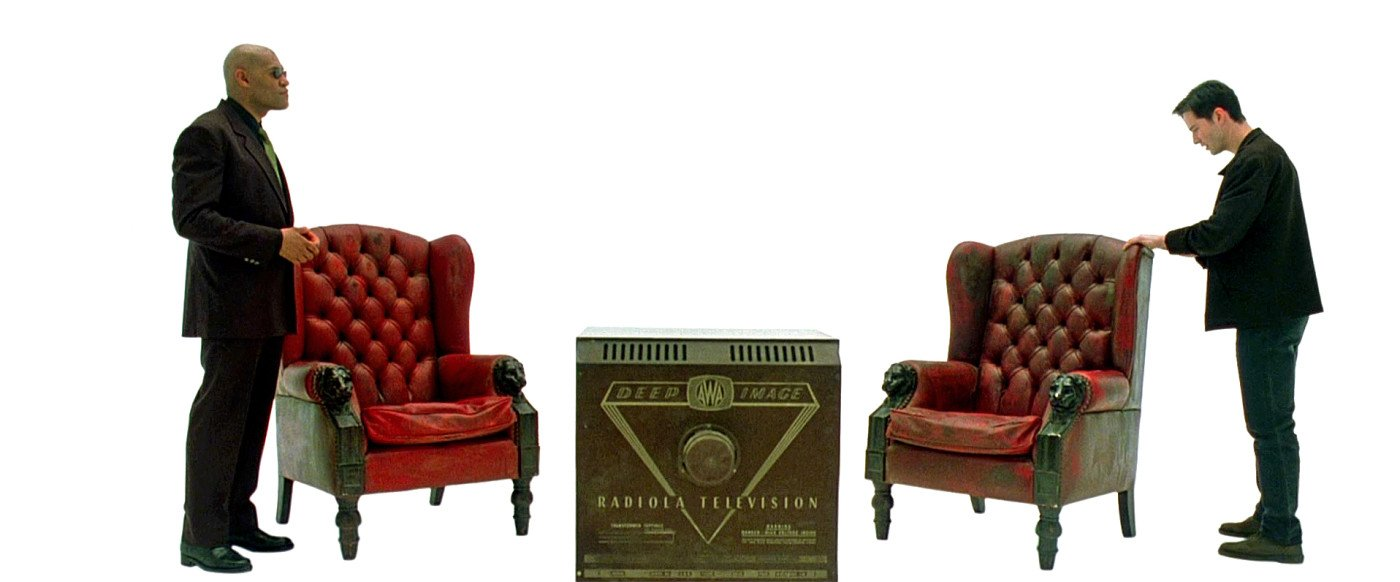
\includegraphics[width=1.0\textwidth]{images/the-matrix-construct3.jpg}
   \end{figure}
   \ \\ \ \\
   \hspace{3cm} `` We can load anything ... anything we need.''
\end{frame}

\begin{frame}
   \frametitle{Containers vs. Virtual Machines}
   \vspace{-4.0em}
   \begin{columns}
      \begin{column}{0.5\textwidth}
         \vspace{5.0em}
         \begin{figure}[htbp]
            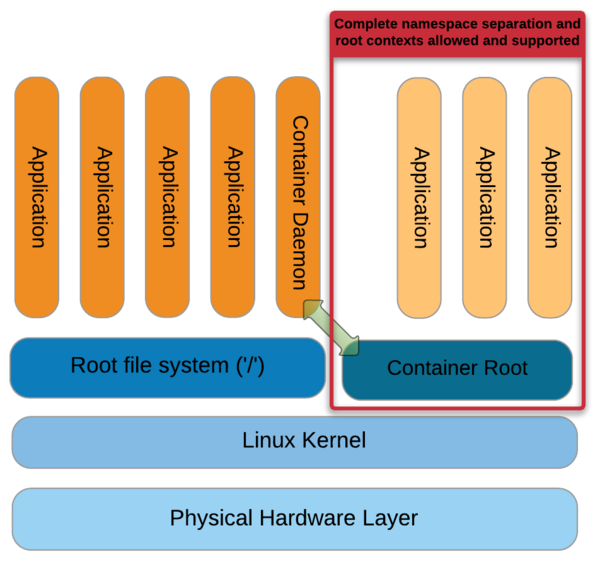
\includegraphics[width=0.9\textwidth]{images/singularity-generic-container-architecture.png}
         \end{figure}
      \end{column}
      \hfill
      \begin{column}{0.5\textwidth}
         \begin{figure}[htbp]
            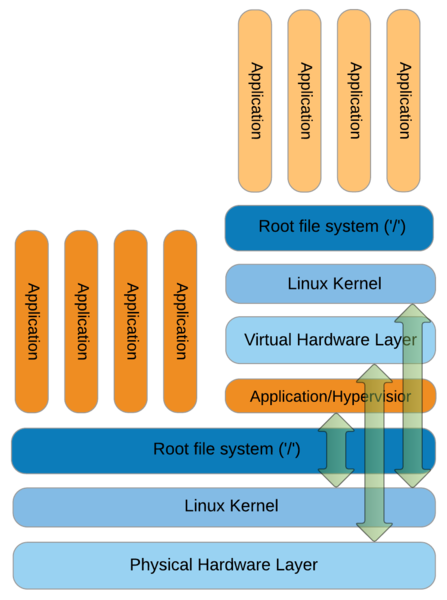
\includegraphics[width=0.9\textwidth]{images/singularity-virtual-machine-architecture.png}
         \end{figure}
      \end{column}
   \end{columns}
   \vspace{1.0em}
   Container-based applications have \textbf{direct access} to the host
   kernel and hardware, \textit{similar to native applications}. In 
   contrast, VM-based applications only have \textbf{indirect access} 
   via the guest OS and hypervisor, which creates a significant 
   \underline{performance overhead}.
\end{frame}

\begin{frame}
   \frametitle{Advantages of Containers}
   \begin{itemize}
      \setlength\itemsep{1.0em}
      \item \textbf{Performance}: Near-native application performance
      \item \textbf{Freedom}: Bring your own software environment
      \item \textbf{Reproducibility}: Package complex software 
         applications into easy to manage, verifiable software units
      \item \textbf{Compatibility}: Built on open standards available in 
         all major Linux distributions
      \item \textbf{Portability}: Build once, run (almost) anywhere 
   \end{itemize}
\end{frame}

\begin{frame}
   \frametitle{Limitations of Containers}
   \begin{itemize}
      \setlength\itemsep{1.0em}
      \item \textbf{Architecture-dependent}: Always limited by CPU 
         architecture (x86\_64, ARM) and binary format (ELF)
      \item \textbf{Portability}: Requires glibc and kernel 
         compatibility between host and container; also requires any 
         other kernel-user space API compatibility (e.g., OFED/IB, 
            NVIDIA/GPUs)
      \item \textbf{Filesystem isolation}: filesystem paths are (mostly) 
         different when viewed inside and outside container
   \end{itemize}
\end{frame}

\begin{frame}
   \frametitle{Docker}
   \begin{columns}
      \begin{column}{0.6\textwidth}
         \begin{itemize}
            \setlength\itemsep{1.0em}
            \item Most common \textbf{container engine} in use today  
            \item Provides tools and utilities to create, maintain, 
               distribute, and run containers images
            \item Designed to accommodate network-centric services (web 
               servers, databases, etc)
            \item Easy to install, well-documentated, and large, 
               well-developed user community and container 
               ecosystem~(DockerHub)
         \end{itemize}
      \end{column}
      \hfill
      \begin{column}{0.5\textwidth}
         \begin{figure}[htbp]
            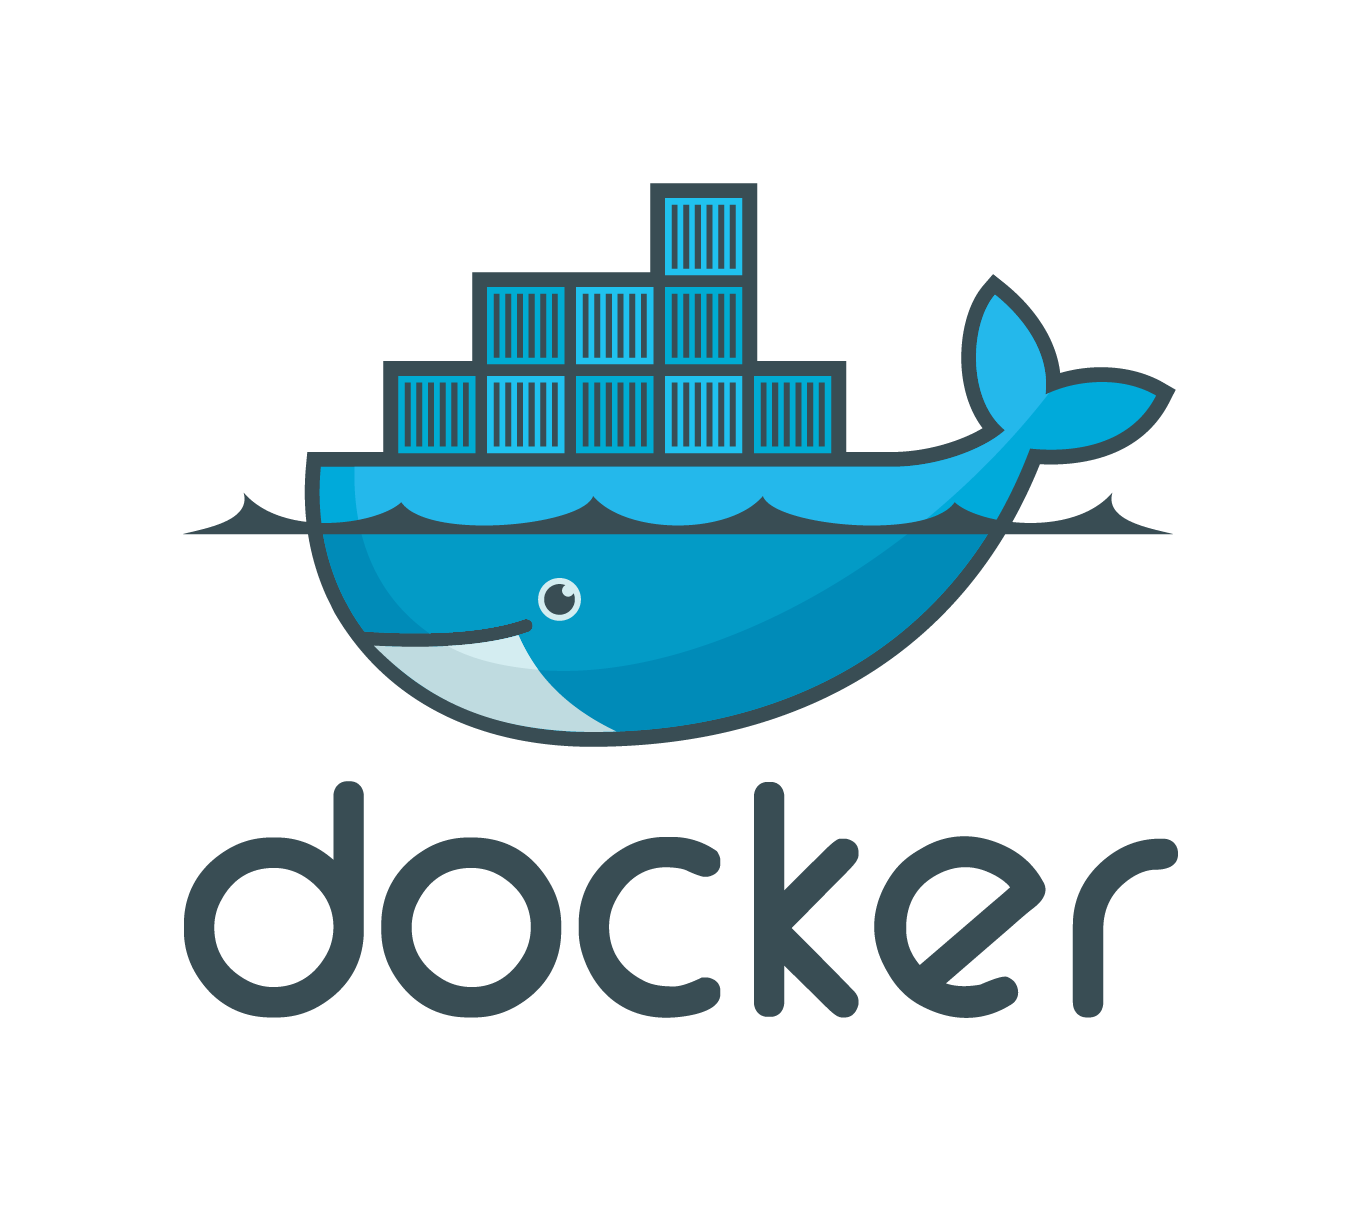
\includegraphics[width=1.0\textwidth]{images/docker-logo.png}
         \end{figure}
         \begin{center}
            \url{https://www.docker.com}
         \end{center}
      \end{column}
   \end{columns}
\end{frame}

\begin{frame}
   \frametitle{Docker on HPC Systems}
   \begin{columns}
      \begin{column}{0.6\textwidth}
      \begin{itemize}
         \setlength\itemsep{1.0em}
         \item HPC systems are shared resources
         \item Docker's security model is designed to support trusted 
            users running trusted containers; e.g., users can escalate to
            root
         \item Docker not designed to support batch-based workflows
         \item Docker not designed to support tightly-coupled, highly
            distributed parallel applications (MPI).
         \end{itemize}
      \end{column}
      \hfill
      \begin{column}{0.5\textwidth}
         \begin{figure}[htbp]
            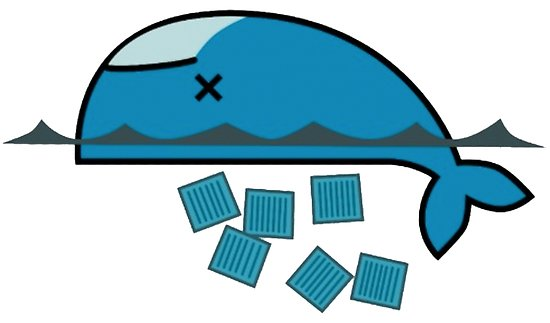
\includegraphics[width=1.0\textwidth]{images/docker-dead-logo.jpg}
         \end{figure}
      \end{column}
   \end{columns}
\end{frame}

\begin{frame}
   \frametitle{Docker on the Cloud (CVE-2019-5736)}
   \begin{columns}
      \begin{column}{0.6\textwidth}
         \begin{itemize}
            \setlength\itemsep{1.0em}
            \item ``The Open Containers Initiative (OCI) recently discovered 
               a new security vulnerability CVE-2019-5736 in runc, allowing 
               container escape to obtain root privileges on the host node.''
            \item `` Amazon employee here: we have released a security 
               bulletin covering how to update to the latest patched 
               Docker on Amazon Linux, Amazon ECS, Amazon EKS, AWS 
               Fargate, AWS IoT Greengrass, AWS Batch, AWS Elastic 
               Beanstalk, AWS Cloud9, AWS SageMaker, AWS RoboMaker, and 
               AWS Deep Learning AMI.''
         \end{itemize}
      \end{column}
      \hfill
      \begin{column}{0.5\textwidth}
         \begin{figure}[htbp]
            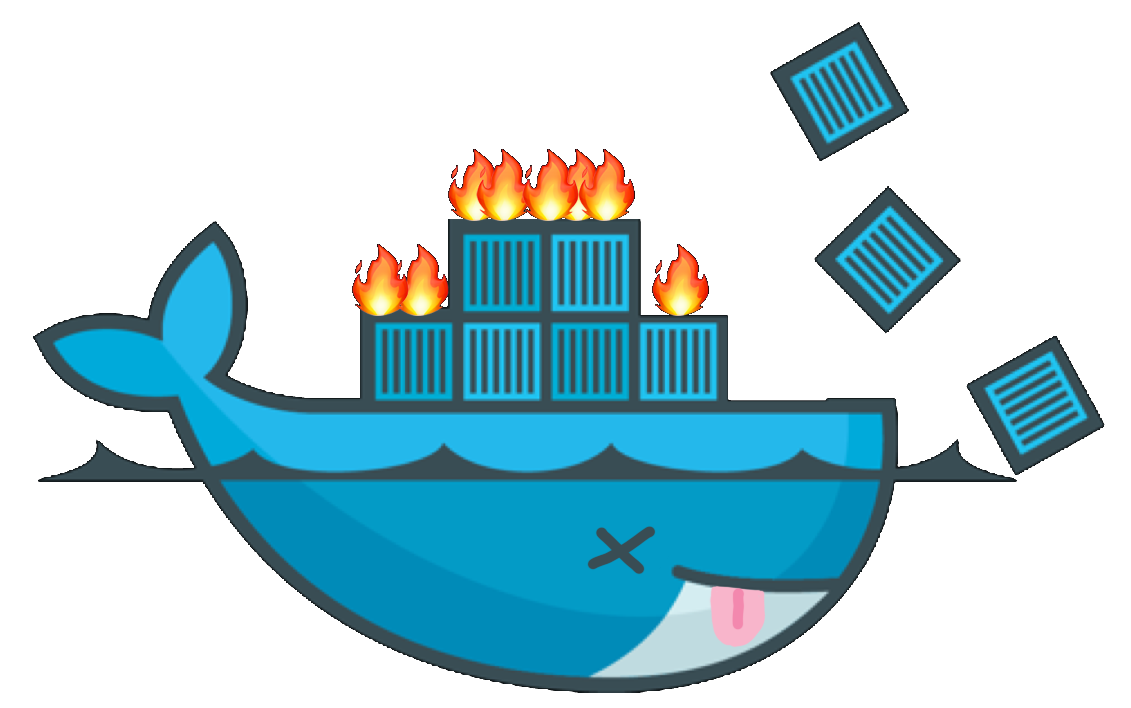
\includegraphics[width=1.0\textwidth]{images/docker-on-fire.png}
         \end{figure}
      \end{column}
   \end{columns}
\end{frame}

\begin{frame}
   \frametitle{Singularity: A Container Engine for HPC}
   \begin{columns}
      \begin{column}{0.6\textwidth}
         \begin{itemize}
            \setlength\itemsep{1.0em}
            \item Reproducible, portable, sharable, and distributable 
               containers
            \item No trust security model: untrusted users running 
               untrusted containers
            \item Support HPC hardware and scientific applications
         \end{itemize}
      \end{column}
      \hfill
      \begin{column}{0.5\textwidth}
         \begin{figure}[htbp]
            
\includegraphics[width=1.0\textwidth]{images/singularity-logo.png}
         \end{figure}
         \begin{center}\small
            \url{http://singularity.lbl.gov}
            \url{https://www.sylabs.io}
         \end{center}
      \end{column}
   \end{columns}
\end{frame}

\begin{frame}
   \frametitle{Features of Singularity}
   \begin{columns}
      \begin{column}{0.6\textwidth}
         \begin{itemize}
            \setlength\itemsep{1.0em}
            \item Each container is a single image file
            \item No root owned daemon processes
            \item No user contextual changes or root escalation allowed; 
               user inside container is always the same user who started 
               the container
            \item Supports shared/multi-tenant resource environments
            \item Supports HPC hardware: Infiniband, GPUs
            \item Supports HPC applications: MPI
         \end{itemize}
      \end{column}
      \hfill
      \begin{column}{0.5\textwidth}
         \begin{figure}[htbp]
            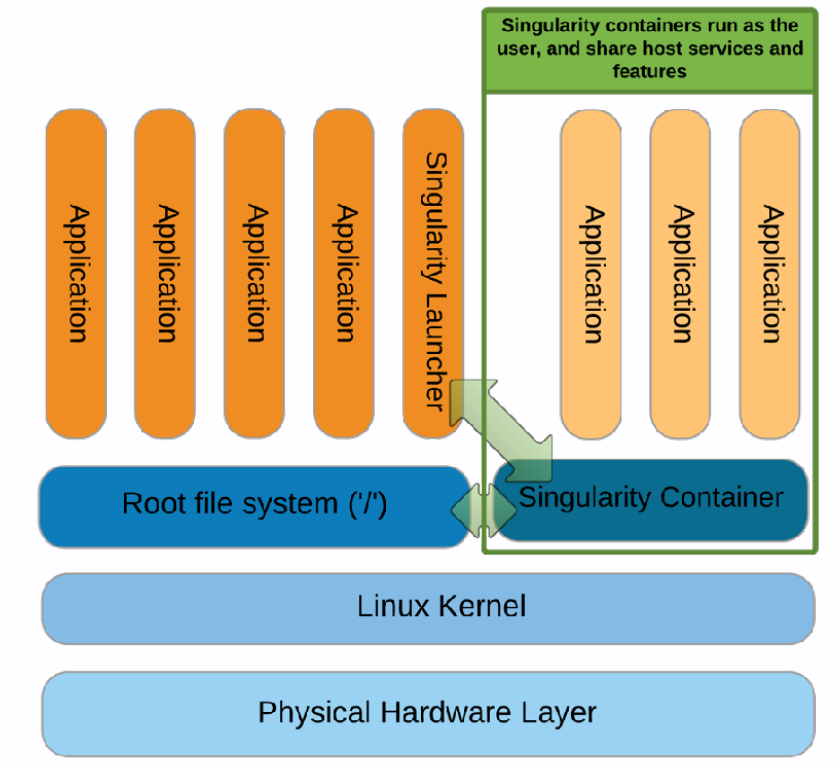
\includegraphics[width=1.0\textwidth]{images/singularity-container-architecture.png}
         \end{figure}
      \end{column}
   \end{columns}
\end{frame}

\begin{frame}
   \frametitle{Common Singularity Use Cases}
   \begin{itemize}
      \setlength\itemsep{1.0em}
      \item Building and running applications that require newer system
         libraries than are available on host system
      \item Running commercial applications binaries that have specific
         OS requirements not met by host system
      \item Converting Docker containers to Singularity containers
   \end{itemize}
\end{frame}

\begin{frame}
   \frametitle{The Singularity Workflow}
   \vspace{-2.0em}
   \begin{columns}
      \begin{column}{0.6\textwidth}
         \begin{enumerate}
            \setlength\itemsep{1.0em}
            \item \textbf{Build} your Singularity containers on a local system 
               where you have root or sudo access; e.g., a personal 
               computer where you have installed Singularity 
            \item \textbf{Transfer} your Singularity containers to the HPC system 
               where you want to run them
            \item \textbf{Run} your Singularity containers on that HPC system
         \end{enumerate}
      \end{column}
      \hfill
      \begin{column}{0.5\textwidth}
         \begin{figure}[htbp]
            
\includegraphics[width=0.4\textwidth]{images/desktop-icon.png}
         \end{figure}
         \vspace{-3.0em}
         \begin{figure}[htbp]
            
\includegraphics[width=0.4\textwidth]{images/file-transfer-arrows.png}
         \end{figure}
         \vspace{-3.0em}
         \begin{figure}[htbp]
            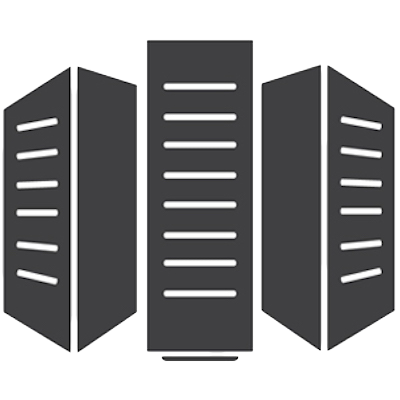
\includegraphics[width=0.4\textwidth]{images/supercomputer-icon.png}
         \end{figure}
      \end{column}
   \end{columns}
\end{frame}

\begin{frame}
   \frametitle{Running Singularity on Mac OS X** or Windows}
   \begin{enumerate}
      \setlength\itemsep{1.0em}
      \item Install VirtualBox on your personal computer: 
         \url{https://www.virtualbox.org}
      \item Create either an Ubuntu or Fedora-based virtual machine, 
         where you will build and test your Singularity containers
      \item Install Singularity* on that virtual machine: 
         \url{https://sylabs.io/guides/3.6/admin-guide/installation.html}
   \end{enumerate}
   \ \\ \ \\
   \footnotesize * Recommendation: Install the same version of 
      Singularity used on the HPC system where you plan to run your 
      containers. If you plan to run on multiple HPC systems, then 
      install the lowest version number you expect to use.
   \ \\ \ \\
   \footnotesize ** Beta Release: \url{https://www.sylabs.io/singularity-desktop-macos}

\end{frame}

\begin{frame}
   \frametitle{Essential Singularity}
   The main Singularity command
   \begin{center}
      \textcolor{blue}{\lstinline{singularity [options] <subcommand> [subcommand options] ...}}
   \end{center}
   has three essential subcommands:
   \begin{itemize}
      \setlength\itemsep{1.0em}
      \item \textcolor{red}{\lstinline{build}}: Build your own container 
         from scratch using a Singularity definition (or recipe) file; 
         download and assemble any existing Singularity container; or 
         convert your containers from one format to another (e.g., from 
         Docker to Singularity)
      \item \textcolor{red}{\lstinline{shell}}: Spawn an interactive shell 
         session in your container.
      \item \textcolor{red}{\lstinline{exec}}: Execute an arbitrary 
         command within your container.
   \end{itemize}
\end{frame}

\begin{frame}
   \frametitle{How to \textit{build} a Singularity container ...}
   ... from a Singularity definition (or recipe) file:
   \begin{figure}[htbp]
      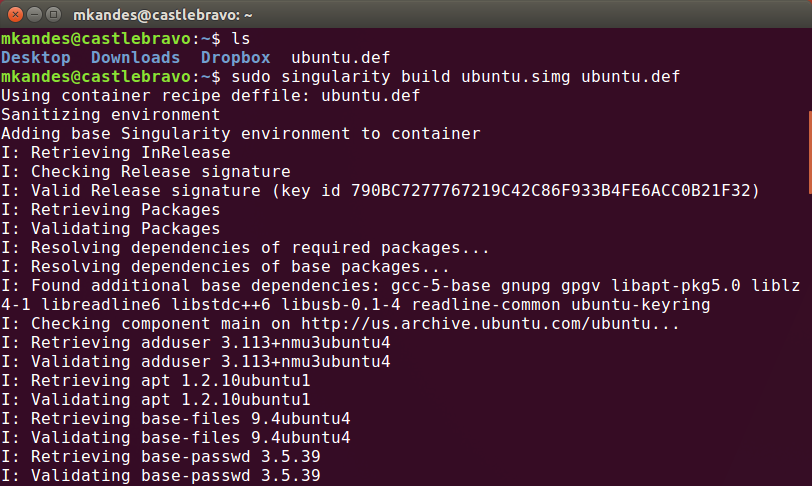
\includegraphics[width=0.8\textwidth]{images/singularity-build-deffile-start.png}
   \end{figure}
   \lstinline{sudo singularity build ubuntu.sif ubuntu.def}
\end{frame}

\begin{frame}
   \frametitle{Singularity Recipe File}
   \begin{columns}
      \begin{column}{0.6\textwidth}
         \begin{itemize}
            \setlength\itemsep{1.0em}
            \item A Singularity definition (or recipe) file is the starting
               point for designing any custom container.
            \item It is a manifest of all software to be installed
               within the container, environment variables to be set,
               files to be added, directories to be mounted,
               container metadata, etc.
            \item You can even write a help section, or define modular
               components in the container.
         \end{itemize}
      \end{column}
      \hfill
      \begin{column}{0.5\textwidth}
         \begin{figure}[htbp]
            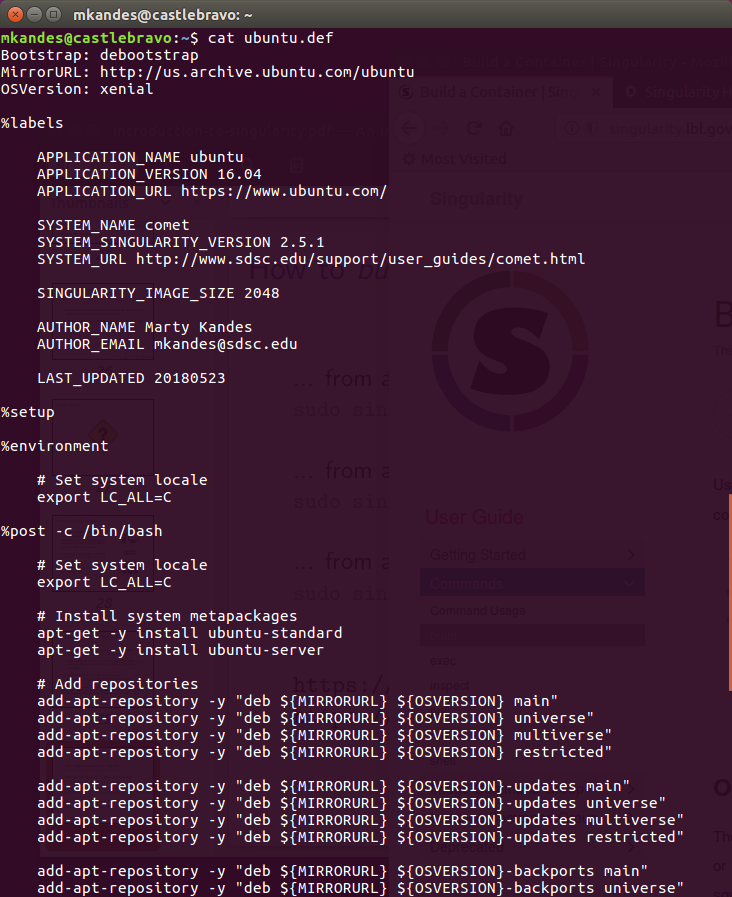
\includegraphics[width=1.0\textwidth]{images/singularity-definition-file.png}
         \end{figure}
      \end{column}
   \end{columns}
\end{frame}

\begin{frame}
   \frametitle{naked-singularity}
   \begin{itemize}
      \setlength\itemsep{1.0em}
      \item A repository of definition (or recipe) files for building
         Singularity containers around the software applications,
         frameworks, and libraries you need to run on high-performance
         computing systems.
      \item Aim of the project is to: \\
      \begin{enumerate}
         \setlength\itemsep{1.0em}
         \item Version control the Singularity containers we're
            building, maintaining, and deploying for you;
         \item Make it easy for you to see what is installed within
            these Singularity containers; and
         \item Make available to you the same base definition files we
            use to build our Singularity containers, which can serve as
            a starting point for your own custom Singularity containers.
      \end{enumerate}
      \item \url{https://github.com/mkandes/naked-singularity}
   \end{itemize}
\end{frame}

\begin{frame}
   \frametitle{How to \textit{build} a Singularity container ...}
   ... from a Singularity definition (or recipe) file:
   \begin{figure}[htbp]
      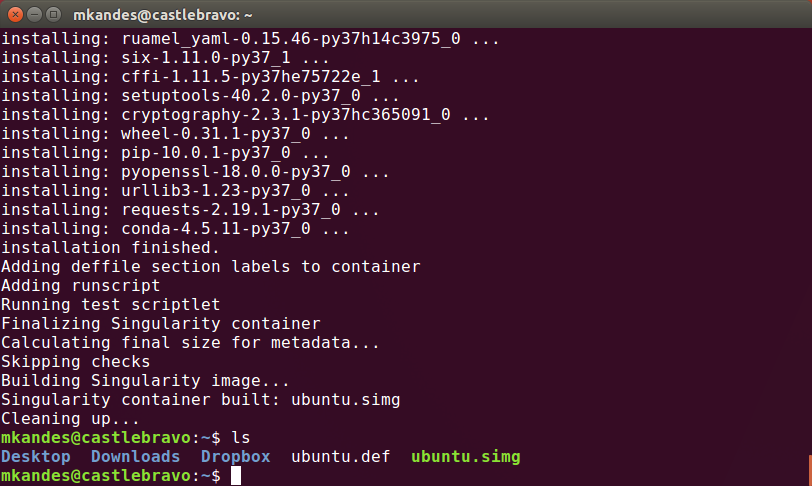
\includegraphics[width=0.8\textwidth]{images/singularity-build-deffile-end.png}
   \end{figure}
   \lstinline{sudo singularity build ubuntu.sif ubuntu.def}
\end{frame}

\begin{frame}
   \frametitle{}
   \begin{figure}[htbp]
      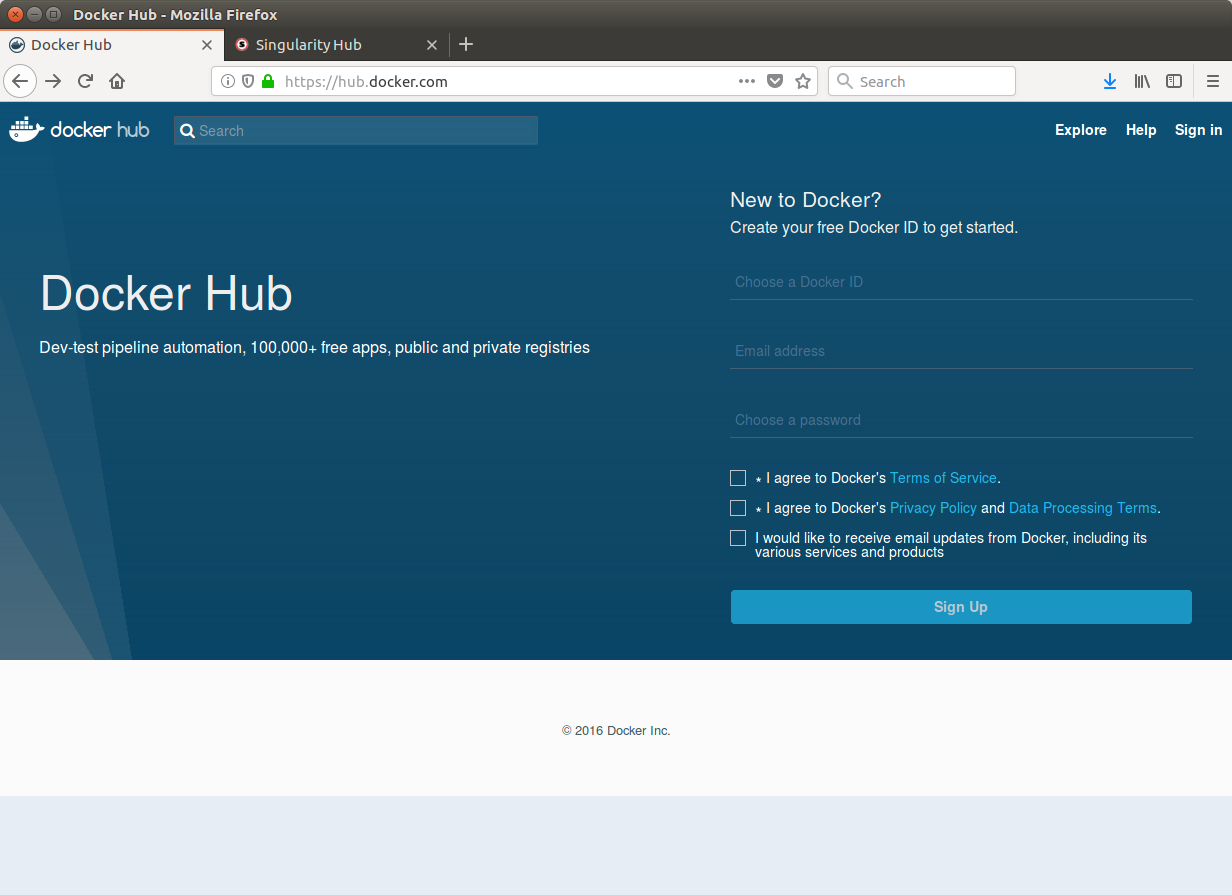
\includegraphics[width=1.0\textwidth]{images/docker-hub-homepage.png}
   \end{figure}
   \begin{center}
      \url{https://hub.docker.com}
   \end{center}
\end{frame}

\begin{frame}
   \frametitle{How to \textit{build} a Singularity container ...}
   ... from an existing Docker container on DockerHub:
   \begin{figure}[htbp]
      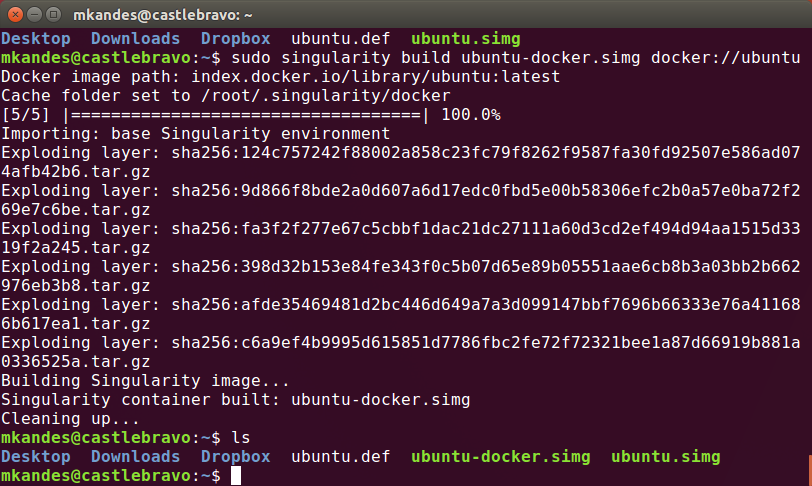
\includegraphics[width=0.8\textwidth]{images/singularity-build-docker.png}
   \end{figure}
   \lstinline{sudo singularity build ubuntu-docker.sif docker://ubuntu}
\end{frame}

\begin{frame}
   \frametitle{}
   \begin{figure}[htbp]
      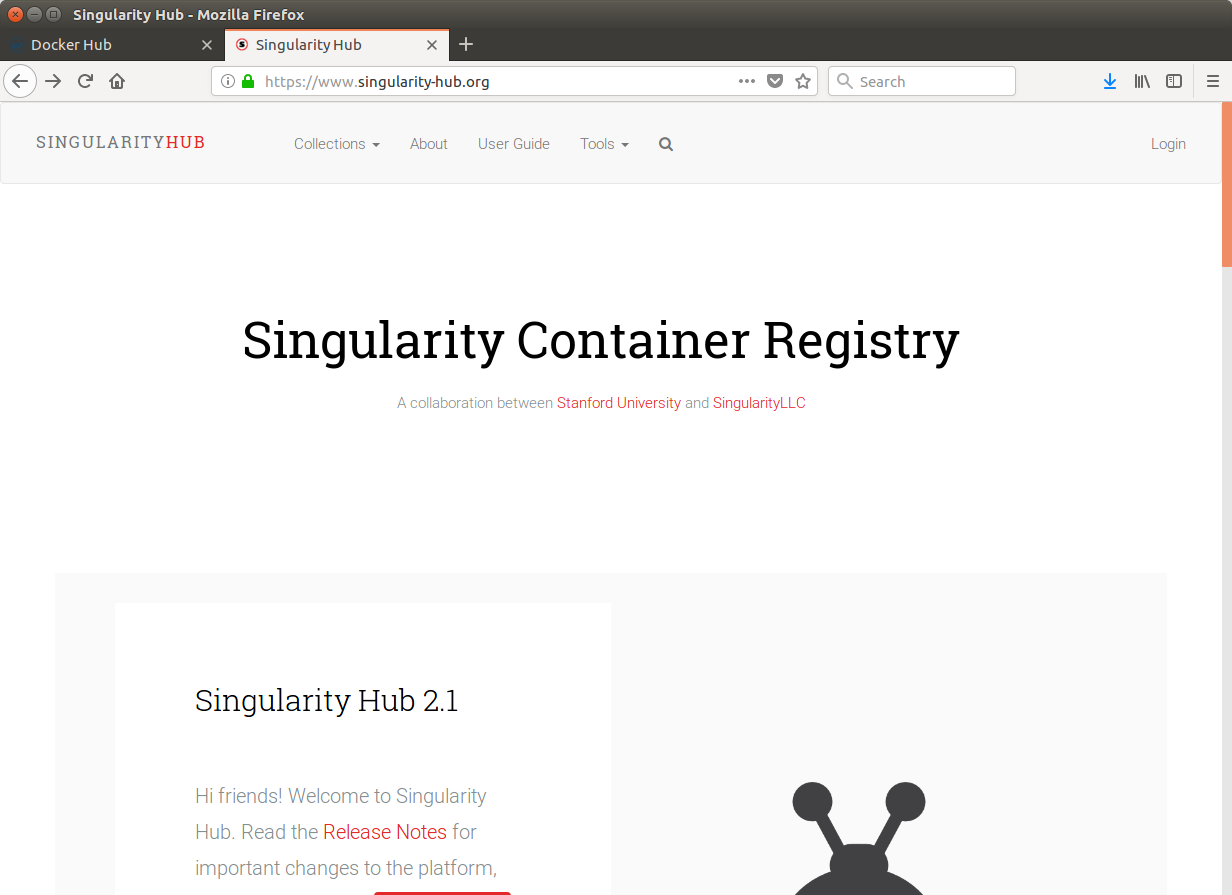
\includegraphics[width=1.0\textwidth]{images/singularity-hub-homepage.png}
   \end{figure}
   \begin{center}
      \url{https://www.singularity-hub.org}
   \end{center}
\end{frame}

\begin{frame}
   \frametitle{How to \textit{build} a Singularity container ...}
   ... from an existing Singularity container on SingularityHub:
   \begin{figure}[htbp]
      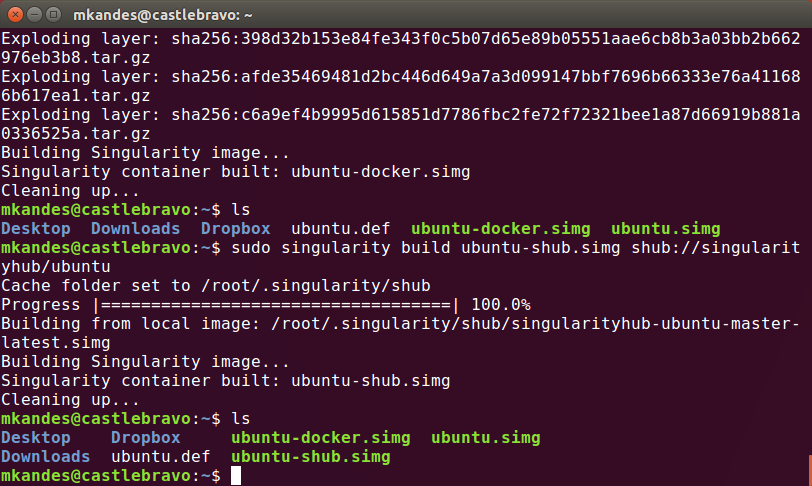
\includegraphics[width=0.8\textwidth]{images/singularity-build-shub.png}
   \end{figure}
   \lstinline{sudo singularity build ubuntu-shub.sif shub://mkandes/ubuntu}
\end{frame}

\begin{frame}
   \frametitle{}
   \begin{figure}[htbp]
      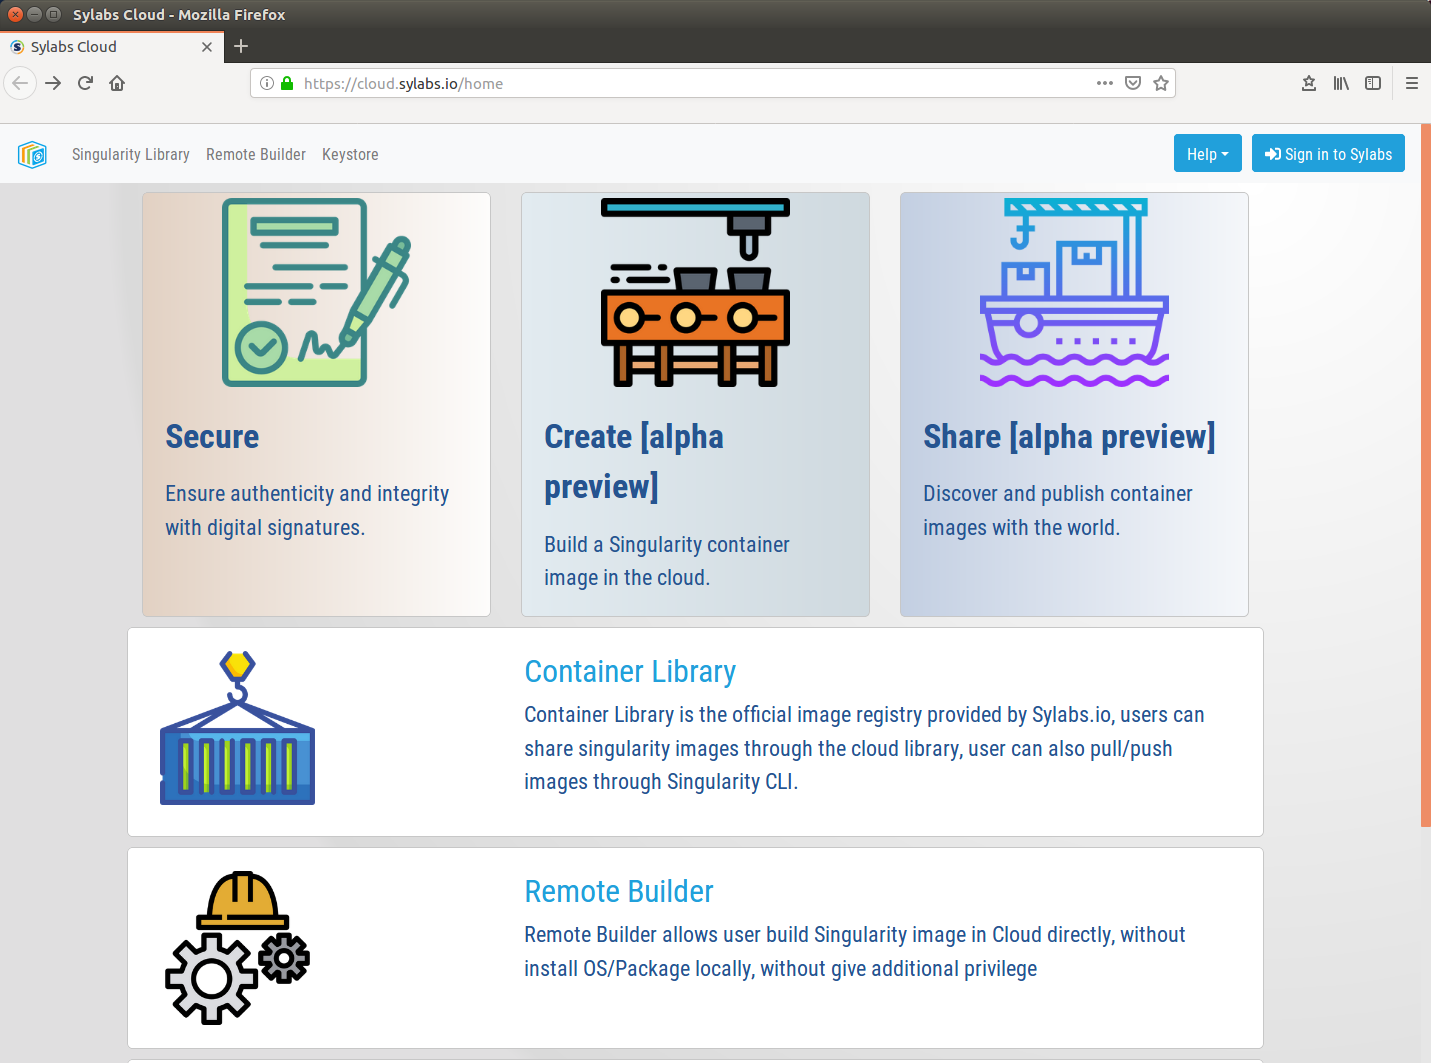
\includegraphics[width=1.0\textwidth]{images/sylabs-cloud.png}
   \end{figure}
   \begin{center}
      \url{https://cloud.sylabs.io}
   \end{center}
\end{frame}

\begin{frame}
   \frametitle{If you \textit{build} it ...}
   \vspace{-1.0em}
   \ \\ \ \\
   \begin{figure}[htbp]
      
\includegraphics[width=0.8\textwidth]{images/field-of-dreams-corn.jpg}
   \end{figure}
   \ \\ \ \\
   \hspace{6cm} ... what can you do with it?
\end{frame}

\begin{frame}
   \frametitle{Essential Singularity}
   The main Singularity command
   \begin{center}
      \textcolor{blue}{\lstinline{singularity [options] <subcommand> [subcommand options] ...}}
   \end{center}
   has three essential subcommands:
   \begin{itemize}
      \setlength\itemsep{1.0em}
      \item \textcolor{green}{\lstinline{build}}: Build your own container
         from scratch using a Singularity definition (or recipe) file;
         download and assemble any existing Singularity container; or
         convert your containers from one format to another (e.g., from
         Docker to Singularity)
      \item \textcolor{red}{\lstinline{shell}}: Spawn an interactive shell
         session in your container.
      \item \textcolor{red}{\lstinline{exec}}: Execute an arbitrary
         command within your container.
   \end{itemize}
\end{frame}

\begin{frame}
   \frametitle{How to spawn an interactive \textit{shell} ...}
   ... within a Singularity container:
   \begin{figure}[htbp]
      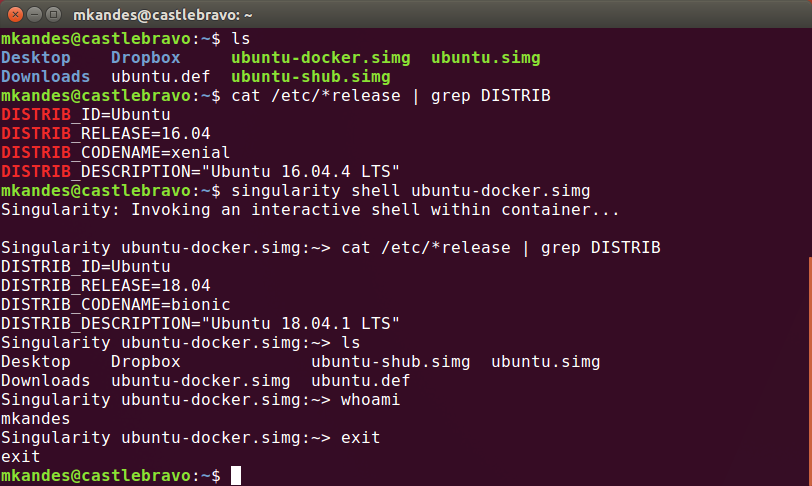
\includegraphics[width=0.8\textwidth]{images/singularity-shell-docker.png}
   \end{figure}
   \lstinline{singularity shell ubuntu-docker.sif}
\end{frame}

\begin{frame}
   \frametitle{Use the interactive \textit{shell} to ... }
   ... explore the software environment of a Singularity container:
   \begin{figure}[htbp]
      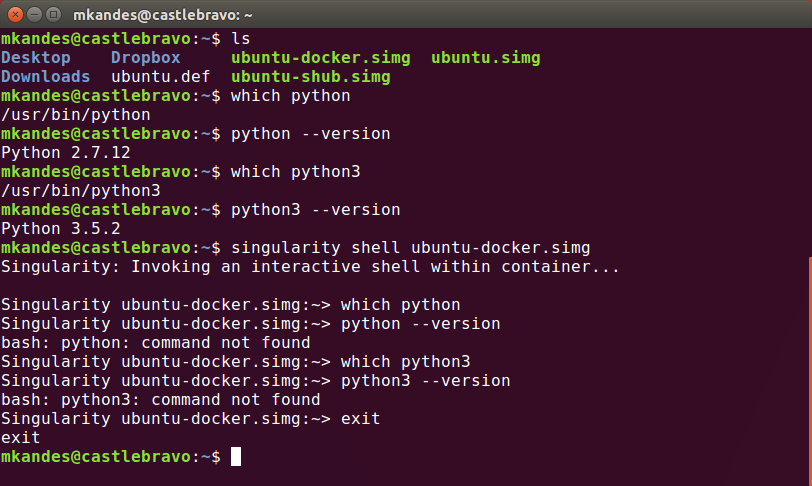
\includegraphics[width=0.8\textwidth]{images/singularity-shell-docker-python.png}
   \end{figure}
   \lstinline{singularity shell ubuntu-docker.sif}
\end{frame}

\begin{frame}
   \frametitle{Use the interactive \textit{shell} to ... }
   ... modify the contents of a Singularity container:
   \begin{figure}[htbp]
      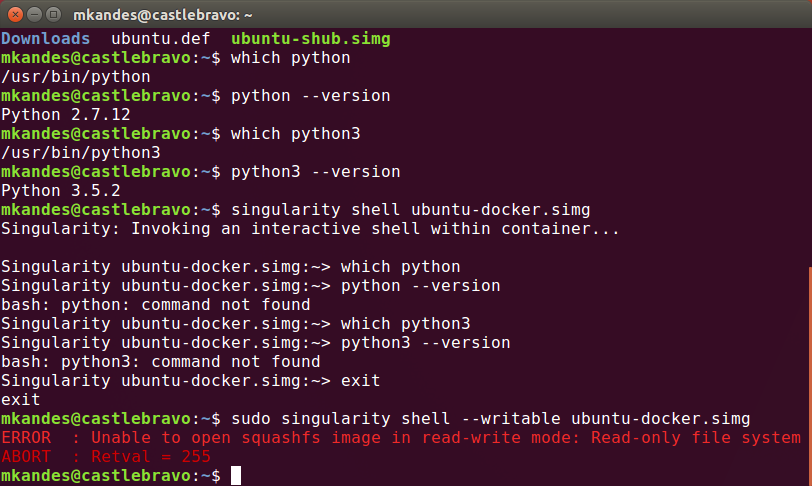
\includegraphics[width=0.8\textwidth]{images/singularity-shell-writable-fail.png}
   \end{figure}
   \lstinline{sudo singularity shell --writable ubuntu-docker.sif}
\end{frame}

\begin{frame}
   \frametitle{}
   \begin{figure}[htbp]
      
\includegraphics[width=0.25\textwidth]{images/do-not-pass-go.png}
   \end{figure}
   \textcolor{red}{\lstinline{ERROR  : Unable to open squashfs image in read-write mode:}} \\
   \textcolor{red}{\lstinline{\ \ \ \ \ \ \ \ \ Read-only file system}} \\
   \textcolor{red}{\lstinline{ABORT  : Retval = 255}}
\end{frame}

\begin{frame}
   \frametitle{Singularity Container Image Formats}
   There are now (only) 2 different Singularity container image formats: 
   \ \\ \ \\
   \begin{itemize}\setlength\itemsep{1.0em}
      \item Compressed READ-ONLY \textbf{Singularity Image File (SIF)} 
         format suitable for production (default)
      \item writable \textbf{(ch)root directory} called a sandbox for 
         interactive (\lstinline{--writable}) development ( --sandbox option)
   \end{itemize}
\end{frame}

\begin{frame}
   \frametitle{How to \textit{build} a \texttt{--sandbox} Singularity container ...}
   ... from an existing Singularity container on SingularityHub:
   \begin{figure}[htbp]
      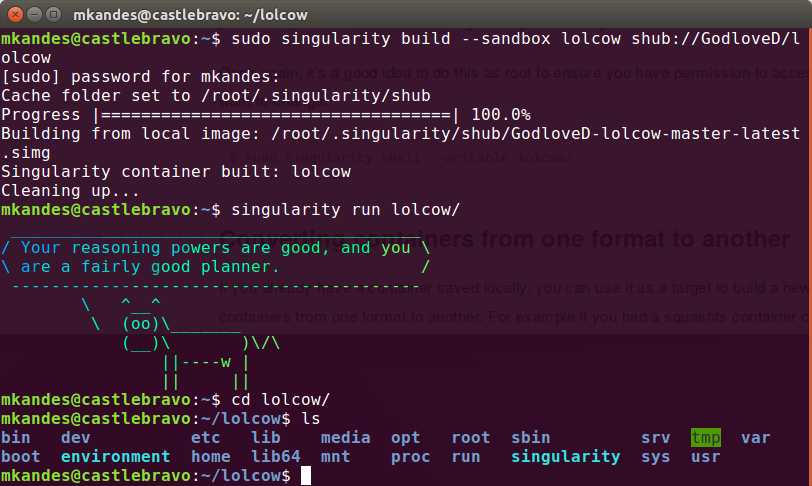
\includegraphics[width=0.8\textwidth]{images/singularity-build-sandbox.png}
   \end{figure}
   \lstinline{sudo singularity build --sandbox lolcow shub://GodloveD/lolcow}
\end{frame}

\begin{frame}
   \frametitle{}
   \vspace{-1.0em}
   \begin{figure}[htbp]
      
\includegraphics[width=1.0\textwidth]{images/now-what.jpg}
   \end{figure}
\end{frame}

\begin{frame}
   \frametitle{Essential Singularity}
   The main Singularity command
   \begin{center}
      \textcolor{blue}{\lstinline{singularity [options] <subcommand> [subcommand options] ...}}
   \end{center}
   has three essential subcommands:
   \begin{itemize}
      \setlength\itemsep{1.0em}
      \item \textcolor{green}{\lstinline{build}}: Build your own container
         from scratch using a Singularity definition (or recipe) file;
         download and assemble any existing Singularity container; or
         convert your containers from one format to another (e.g., from
         Docker to Singularity)
      \item \textcolor{green}{\lstinline{shell}}: Spawn an interactive shell
         session in your container.
      \item \textcolor{red}{\lstinline{exec}}: Execute an arbitrary
         command within your container.
   \end{itemize}
\end{frame}

\begin{frame}
   \frametitle{How to \textit{exec}ute ... }
   ... arbitrary commands within a Singularity container:
   \begin{figure}[htbp]
      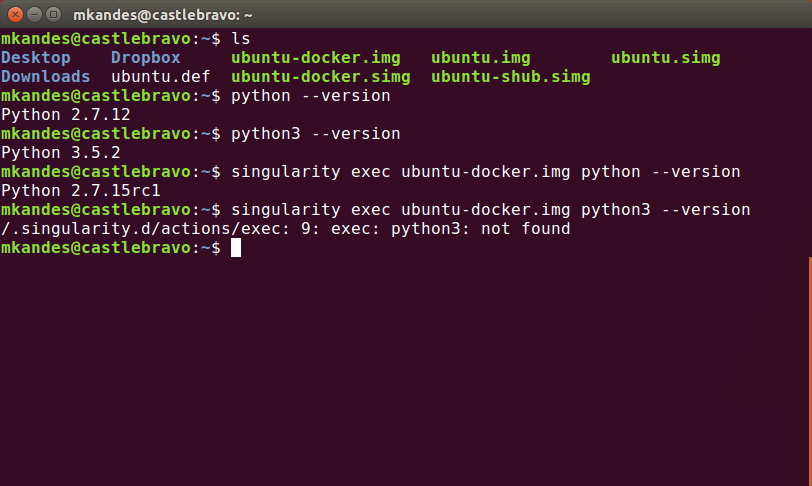
\includegraphics[width=0.8\textwidth]{images/singularity-exec-python-version-check.png}
   \end{figure}
   \lstinline{singularity exec ubuntu-docker.img python --version}
\end{frame}

\begin{frame}
   \frametitle{Essential Singularity}
   The main Singularity command
   \begin{center}
      \textcolor{blue}{\lstinline{singularity [options] <subcommand> [subcommand options] ...}}
   \end{center}
   has three essential subcommands:
   \begin{itemize}
      \setlength\itemsep{1.0em}
      \item \textcolor{green}{\lstinline{build}}: Build your own container
         from scratch using a Singularity definition (or recipe) file;
         download and assemble any existing Singularity container; or
         convert your containers from one format to another (e.g., from
         Docker to Singularity)
      \item \textcolor{green}{\lstinline{shell}}: Spawn an interactive shell
         session in your container.
      \item \textcolor{green}{\lstinline{exec}}: Execute an arbitrary
         command within your container.
   \end{itemize}
\end{frame}

\begin{frame}
   \frametitle{MPI-based Singularity Containers}
   \begin{columns}
      \begin{column}{0.6\textwidth}
         \begin{itemize}
            \setlength\itemsep{1.0em}
            \item Use same Message Passing Interface~(MPI) distribution
               and version within container as would be used outside the
               container.
            \item If using Infiniband~(IB), install same OFED drivers and
               libraries inside the container as used on underlying HPC
               hardware.
         \end{itemize}
      \end{column}
      \hfill
      \begin{column}{0.5\textwidth}
         \begin{figure}[htbp]
            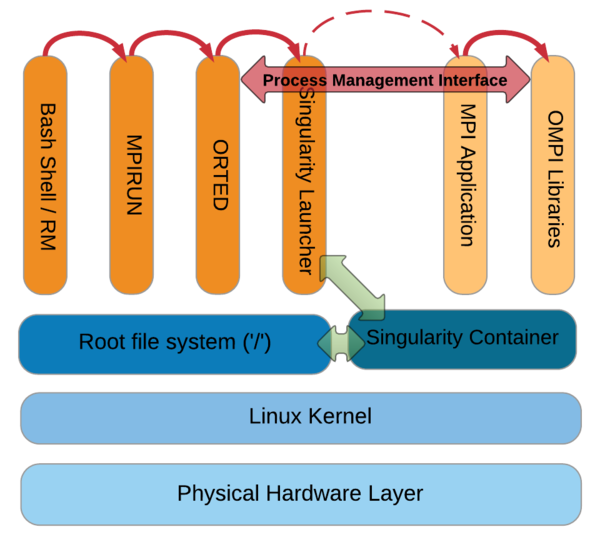
\includegraphics[width=1.0\textwidth]{images/singularity-container-architecture-with-mpi.png}
         \end{figure}
      \end{column}
   \end{columns}
\end{frame}

\begin{frame}
   \frametitle{MPI-based Singularity Containers: MEEP}
   \begin{columns}
      \begin{column}{0.6\textwidth}
         \begin{itemize}
            \setlength\itemsep{1.0em}
            \item MEEP: MIT Electromagnetic Equation Propagation is a 
               free and open-source software package for simulating 
               electromagnetic systems via the finite-difference 
               time-domain (FDTD) method.
            \item Dependency hell: Too difficult to compile in TSCC's 
               native software environment.
         \end{itemize}
      \end{column}
      \hfill
      \begin{column}{0.5\textwidth}
         \begin{figure}[htbp]
            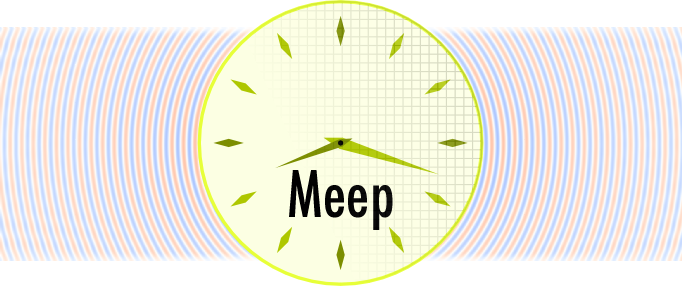
\includegraphics[width=1.0\textwidth]{images/meep-logo.png}
         \end{figure}
      \end{column}
   \end{columns}
\end{frame}

\begin{frame}
   \frametitle{MPI-based Singularity Containers: MEEP}
   \begin{figure}[htbp]
      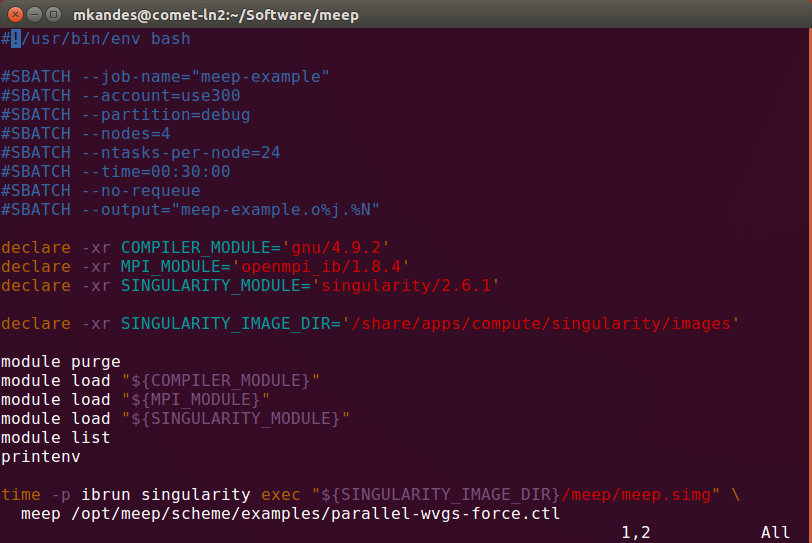
\includegraphics[width=0.8\textwidth]{images/meep-singularity-mpi-example-batch-job.png}
   \end{figure}
   \lstinline{mpirun -np X singularity exec meep.sif meep parallel-wvgs-force.ctl}
\end{frame}

\begin{frame}
   \frametitle{GPU-accelerated Singularity Containers}
   \begin{columns}
      \begin{column}{0.6\textwidth}
         \begin{itemize}
            \setlength\itemsep{1.0em}
            \item GPU-accelerated containers also require an interface 
               for accessing GPU drivers and libraries on the underlying 
               host system.
            \item Traditionally, you would install the same driver and 
               libraries within container that match distribution and version
               of them available on the host system.
            \item Today, Singularity actually allows you to bind mount 
               the GPU driver and its supporting libraries at runtime 
               with the \texttt{--nv} option. 
         \end{itemize}
      \end{column}
      \hfill
      \begin{column}{0.5\textwidth}
         \begin{figure}[htbp]
            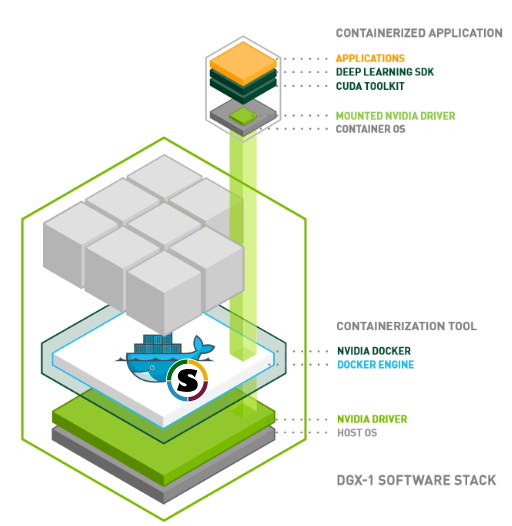
\includegraphics[width=1.0\textwidth]{images/nvidia-docker-stack+singularity.png}
         \end{figure}
      \end{column}
   \end{columns}
\end{frame}

\begin{frame}
   \frametitle{GPU-accelerated Singularity Containers: TensorFlow}
   \begin{columns}
      \begin{column}{0.6\textwidth}
         \begin{itemize}
            \setlength\itemsep{1.0em}
            \item TensorFlow is an open source software library for high 
               performance numeric and symbolic computation, and is most 
               popularly used today for machine learning applications 
               such as neural networks. 
            \item Like many of the most popular machine learning 
               frameworks, TensorFlow continues to evolve rapidly. At 
               present, the latest versions of TensorFlow are 
               incompatible with the version of TSCC's \texttt{glibc} 
               library.
         \end{itemize}
      \end{column}
      \hfill
      \begin{column}{0.5\textwidth}
         \begin{figure}[htbp]
            
\includegraphics[width=1.0\textwidth]{images/tf_logo_social.png}
         \end{figure}
      \end{column}
   \end{columns}
\end{frame}

\begin{frame}
   \frametitle{GPU-accelerated Singularity Containers: TensorFlow}
   \begin{figure}[htbp]
      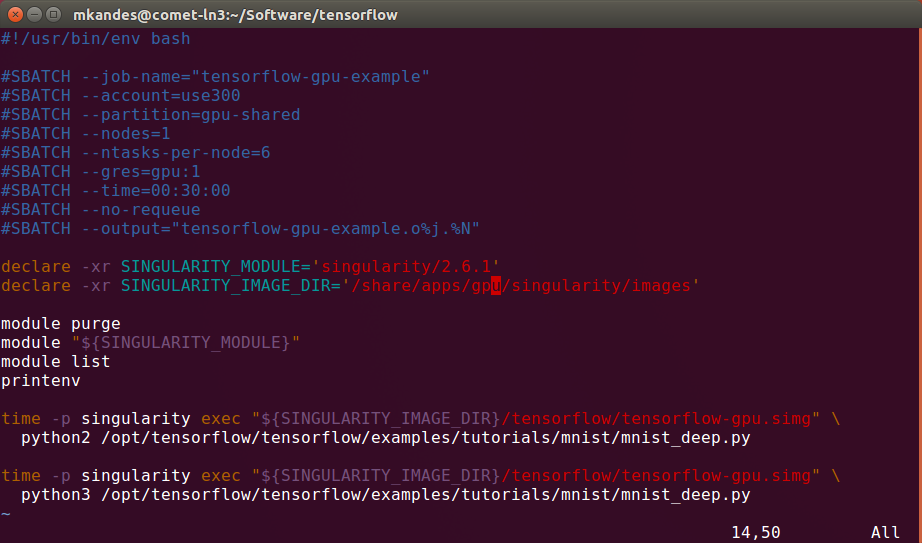
\includegraphics[width=0.8\textwidth]{images/tensorflow-singularity-gpu-example-batch-job.png}
   \end{figure}
   \lstinline{singularity exec keras-tensorflow-gpu.sif python mnist\_deep.py}
\end{frame}

\begin{frame}
   \frametitle{GPU-accelerated Singularity Containers: TensorFlow}
   \begin{figure}[htbp]
      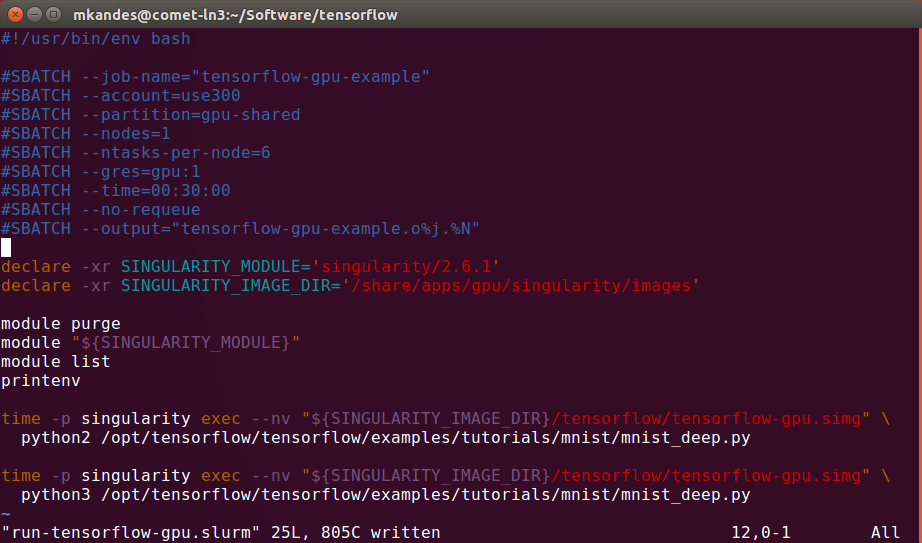
\includegraphics[width=0.8\textwidth]{images/tensorflow-singularity-gpu-example-batch-job-with--nv.png}
   \end{figure}
   \lstinline{singularity exec --nv keras-tensorflow-gpu.sif python mnist\_deep.py}
\end{frame}

\begin{frame}
   \frametitle{Exoskeletal (Dependency-Only) Singularity Containers}
   \begin{itemize}
      \setlength\itemsep{1.0em}
      \item Some software applications may need to be installed in your 
         \$HOME directory on the underlying host system, but may require 
         software dependencies not available and/or not supported on the 
         host system. e.g., Julia with GPU support.
      \item Most often, users simply want to install additional packages 
         in the Singularity containers we build and maintain for you.
      \item In both cases, the you can use any container's environment to 
         install the software you need to in your \$HOME directory. 
         Note, however, this can create some dependency confusion down 
         the road when you forget which packages were installed with 
         what container. 
   \end{itemize}
   \lstinline{singularity exec ubuntu.sif pip install --user networkx}
\end{frame}

\begin{frame}
   \frametitle{Singularity: A Summary}
   \begin{enumerate}
      \setlength\itemsep{1.0em}
      \item You can now install (almost) any software you like on your 
         favorite HPC system without having to make a special request 
         to the system's administrators or user support staff.
      \item In many cases, your software is now completely portable 
         between the different HPC systems you want to run on.
      \item And finally, you now have discrete software units 
         (containers) that you can use to help maintain science 
         reproducibility over the lifetime of a project, independent of 
         how the software environment on any given HPC system changes 
         over time.
   \end{enumerate}
\end{frame}

\begin{frame}
   \frametitle{Questions?}
   \vspace{-1.0em}
   \begin{figure}[htbp]
      
\includegraphics[width=0.5\textwidth]{images/homer-simpson-glasses.jpg}
   \end{figure}
\end{frame}

\end{document}
